\documentclass{beamer}
\usepackage[latin1]{inputenc}
%\usetheme[noshadow,nonav,nologo]{NYU}
\usetheme[numbers]{NYU}
\usepackage{amsmath}
\usepackage{amsfonts}
\usepackage{amssymb}

\title{Factorization of High Dimensional Data using a Temporal Auto-Encoder Framework}
\date{December 18, 2013} 
\author{Ross Goroshin \hspace{0.20cm} Joan Bruna \hspace{0.20cm} Arthur Szlam}


\begin{document}

\begin{frame}
\titlepage
\end{frame}

\begin{frame}
\frametitle{Structure in Natural Data \& Statistical Dependence}  
\begin{center}
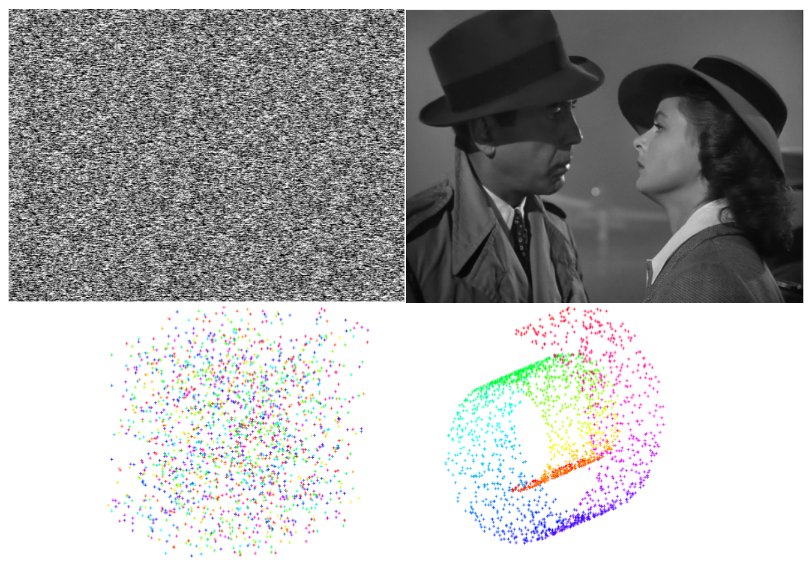
\includegraphics[scale=0.2]{./figures/structure.png}
\begin{itemize} 
\item Suppose we have a 42 second video played at 24 frames/second, with a resolution of 1000 by 1000 pixels
\item In theory each pixel can vary independently from frame to frame, which implies that there are $\approx 10^9$ degrees of freedom 
\item If all pixels in natural images were i.i.d then natural images would fill the space. Sampling from this distribution would produce natural images.
\end{itemize} 
\end{center}
\end{frame}

\begin{frame} 
\frametitle{Structure in Natural Data \& Statistical Dependence}
\begin{center} 
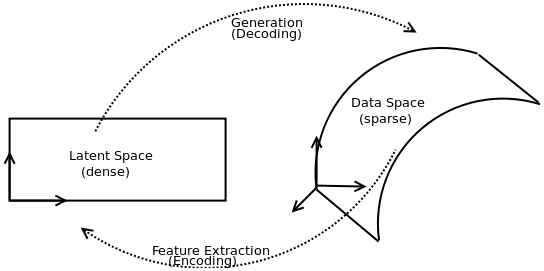
\includegraphics[scale = 0.5]{./figures/spaces.png}
\end{center} 
\begin{itemize} 
\item This illustration is representative of many processes 
\item However, dependence can be introduced without increasing the dimensionality 
\item Latent representation is NOT unique for generative processes of interest
\end{itemize}  
\end{frame}

\begin{frame}
\frametitle{Unsupervised Learning} 
\begin{itemize}
\item Unsupervised learning algorithms should, in some sense, \emph{parameterize} the data manifold 
\item These parameters are referred to as \emph{features or factors} 
\item A good feature representation should satisfy the following criteria: (1) the features are mutually independent, (2) the representation is \emph{not one that is invariant} but \emph{linearly equivariant} to the set of transformation groups present in the data. This makes it possible to formulate any classification, detection, or regression task as a linear problem in feature space. Finally, (3) because we do not know the task a priori, the represntation should be loss-less, i.e. is information preserving.  
\end{itemize} 
\end{frame} 

\begin{frame}
\frametitle{Dimensionality Reduction by Learning an Invariant Mapping (DrLIM)} 
\begin{itemize}
\item{We wish to find a mapping $G_W(X_i): \mathbb{R}^D \rightarrow \mathbb{R}^d$, where $D>d$ which translates labeled similarity relationships in the input space to Euclidean distances in the output space} 
\item{If $(X_1, X_2)$ are similar then $Y=0$, otherwise $Y=1$}
\item{Let $D_W(X_1, X_2) = \|G_W(X_1),G_W(X_2)\|_2$}
\item{$L(W,Y,X_1,X_2) = (1-Y)\frac{1}{2}D_W^2 + Y \frac{1}{2}\{max(0,m-D_W)\}^2$}   
\begin{center}
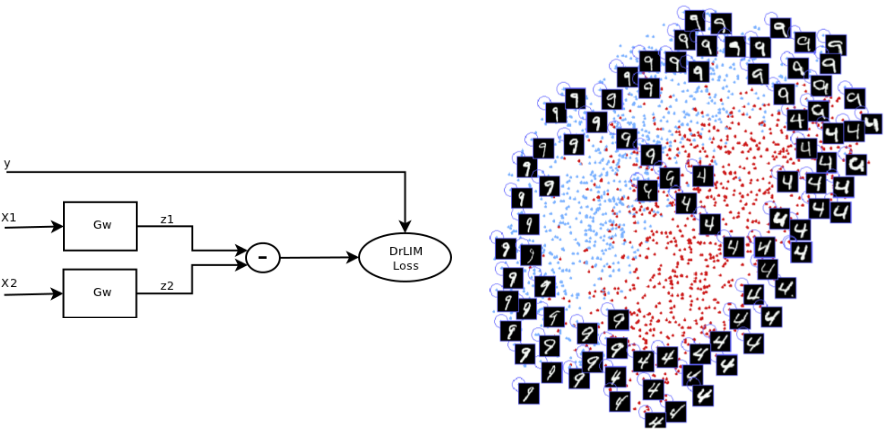
\includegraphics[scale = 0.3]{./figures/drlim_mnist.png}  
\end{center} 
\end{itemize} 
\end{frame} 

\begin{frame}
\frametitle{Unsupervised Feature Learning with DrLIM}
Although DrLIM can be used to extract some of the underlying factors that describe a high-dimensional dataset, there are several limitations which preclude it from being a general purpose feature learning algorithm.  
\begin{itemize}
\item Where do we obtain the similarity labels $Y$?
\item DrLIM does not include a reconstruction cost, and thus produces a non-invertible (lossy) feature set, i.e. the mapping $G_w()$ is trained to be invariant 
\item The features extracted are not guaranteed to be independent (factorized representation). This becomes a problem as the number of features increases
\end{itemize}
\end{frame}

\begin{frame}
\frametitle{Problem 1 or 3: Similarity Labels and the Role of Time}
\center
\begin{itemize}
\item{If the objects in consecutive frames do not overlap then all samples are equidistant from each other}
\item{\emph{Without prior knowledge}, meaningful neighborhood relationships can only be deduced from temporally coherent sequences of images (i.e. movie clips)}
\end{itemize}
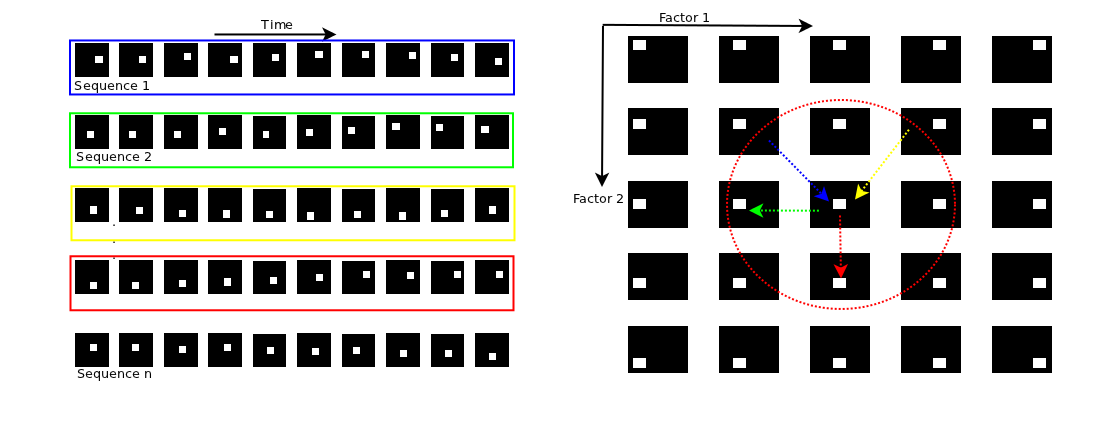
\includegraphics[scale = 0.25]{./figures/diagram1.png} 
\end{frame}

\begin{frame} 
\frametitle{DrLIM Applied to Temporally Coherent Data}
\begin{center} 
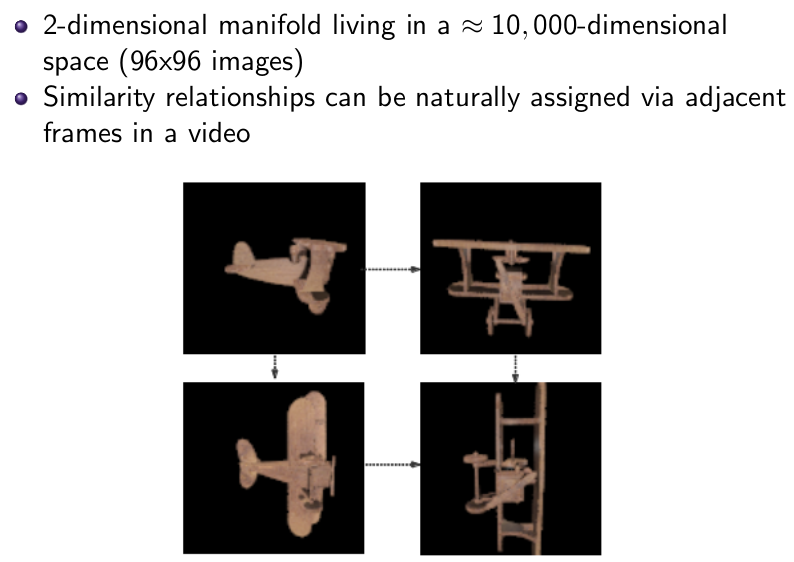
\includegraphics[scale = 0.25]{./figures/drlim_data.png} 
\end{center} 
\begin{center} 
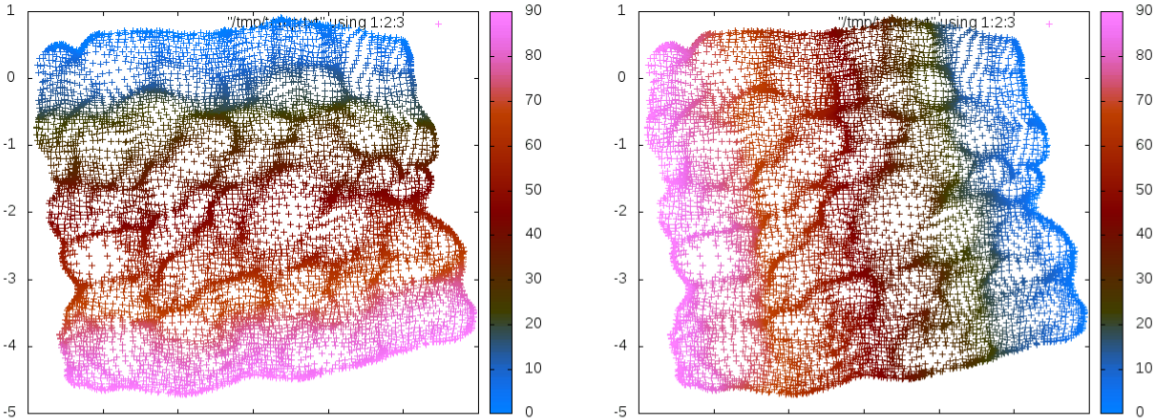
\includegraphics[scale = 0.15]{./figures/drlim_result.png} 
\end{center} 
\end{frame} 

\begin{frame} 
\frametitle{Problem 2 of 3: \emph{Invariance VS Equivariance}}
\begin{itemize}
\item The mapping $G_w()$ is trained to extract the underlying factors which generate a particular temporal sequence 
\item However, this mapping is trained to be invariant to any other variations that may be present in the data     
\item The mapping $G_w()$ is \emph{not necessarily invertible}, thus it is not information preserving 
\end{itemize} 
\end{frame} 

\begin{frame}
\frametitle{DrLIM + Reconstruction Loss} 
\begin{center} 
\begin{itemize}
\item $Gw()$ and $Rw()$ are trainable functions called the 'encoder' and 'decoder', respectively
\item $z_i$ is an intermediate, high dimensional representation 
\item $U$ is a trainable \emph{linear} map
\end{itemize}
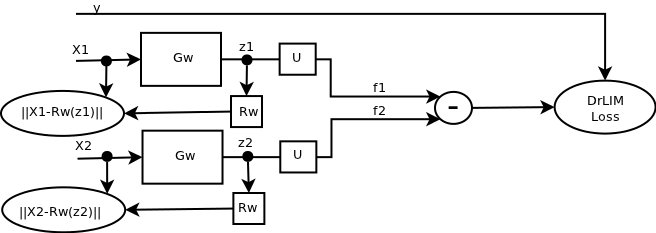
\includegraphics[scale = 0.4]{./figures/redrlim_diag.png} 
\vspace{0.7cm}
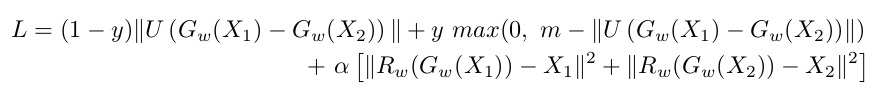
\includegraphics[scale = 0.3]{./figures/redrlim_loss.png} 
\end{center} 
\end{frame} 

\begin{frame}
\frametitle{DrLIM + Reconstruction Loss} 
\begin{itemize}
\item Encoder has two stages: $z=G_w(X)$ and $f=Uz$
\item The representation $z$ is one from which we can: (i) reconstruct the input and (ii) linearly extract the factors of variation 
\item Thus $z$ is a factorized representation in which the factors have been disentangled from the rest of the information
\end{itemize} 
\begin{center}
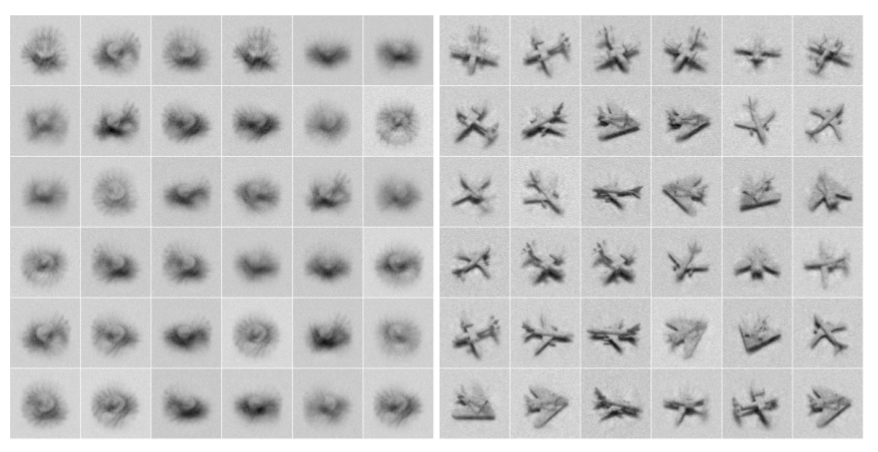
\includegraphics[scale = 0.3]{./figures/redrlim.png} 
\end{center} 
\end{frame} 

\begin{frame}
\frametitle{A Simpler Experiment} 
\begin{center} 
\begin{itemize}
\item Assume that $G_w()$ produces a large (over-complete) feature set
\item $z = [X~f]$ is a possible solution to the unregularized network. Where $f$ are the relavant features for the supervised task
\item Since $f$ is causally extracted from $X$ they are not independent
\end{itemize}

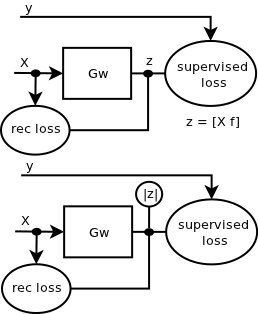
\includegraphics[scale = 0.4]{./figures/inv_vs_eqi.png} 
\end{center} 
\end{frame} 

\begin{frame}
\frametitle{Problem 3 of 3: Promoting Independent Features}  
\begin{itemize}
\item A 'factorized' representation implies that the features extracted are independent
\item Independence can be encouraged by maximizing the sparsity of $z_1 - z_2$ 
\item This means that only a small number of features change between adjacent video frames
\item Use a sparifying norm $\|z_1-z_2\|_p$ where $p \leq 1$    
\end{itemize}
\end{frame} 

\begin{frame}
\frametitle{Slow, Sparse Transition Features} 
\begin{itemize}
\item $|z_1 - z_2|_1$ not only encourages the features to vary slowly in time, but also encourages $z_1 - z_2$ to be as sparse as possible
\item This is also called the total-variation (TV-norm)  
\item The implicit prior corresponding to this penalty is that \emph{only a small set of latent factors vary between adjacent frames}
\end{itemize}
\begin{center}
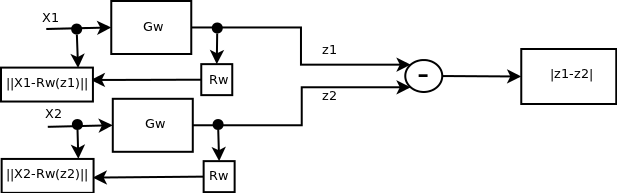
\includegraphics[scale = 0.4]{./figures/sfa_diag.png} 
\end{center} 
\end{frame} 

\begin{frame}
\frametitle{Slow Features Experiment \#1}   
\begin{columns}[c]
    \column{2.5cm}
        %\begin{center}
            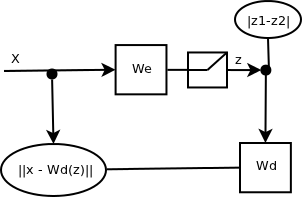
\includegraphics[scale=0.3]{./figures/sfa2.png} 
            \vspace{0.1cm}
             \begin{tiny}
			 Encoder: ReLU \\
			 Decoder: Norm Linear
			\end{tiny}
        %\end{center}
    \column{3cm}
        \begin{center} 
        $L_1$
             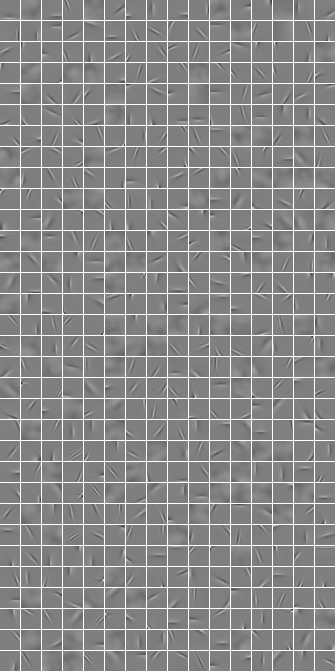
\includegraphics[scale=0.3]{./figures/L1.png}
        \end{center}
     \column{3cm} 
     \begin{center} 
     $SF$ 
     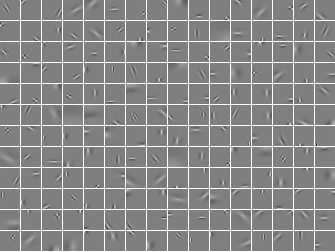
\includegraphics[scale=0.3]{./figures/SF.png} 
     \end{center} 
     
\end{columns} 
\end{frame} 

\begin{frame}
\frametitle{Slow Features Experiment \#2}    
\begin{columns}[c]
    \column{4cm}
        %\begin{center}
            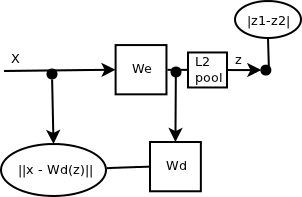
\includegraphics[scale=0.3]{./figures/sfa3.png} 
            \vspace{0.1cm}
             \begin{tiny}
			 Encoder: Linear \\
			 Decoder: Norm Linear \\
			 $L_2$-pooling: $z_{11} = \sqrt{\sum_{i=1} ^4 (W^e_i x)^2}$
			\end{tiny}
        %\end{center}
    \column{4cm}
        %\begin{center}
             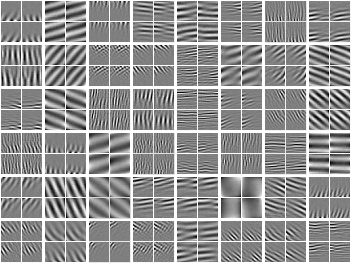
\includegraphics[scale=0.3]{./figures/fourier.png} 
        %\end{center}
\end{columns} 
\end{frame} 

\begin{frame}
\frametitle{Slow Features Experiment \#3}    
\begin{columns}[c]
    \column{4cm}
        %\begin{center}
            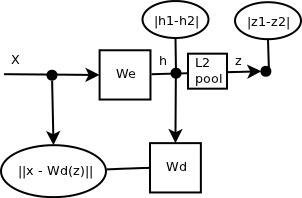
\includegraphics[scale=0.3]{./figures/sfa4.png} 
            \vspace{0.1cm}
             \begin{tiny}
			 Encoder: Linear \\
			 Decoder: Norm Linear \\
			 $L_2$-pooling: $z_{11} = \sqrt{\sum_{i=1} ^4 (W^e_i x)^2}$
			\end{tiny}
        %\end{center}
    \column{4cm}
        %\begin{center}
             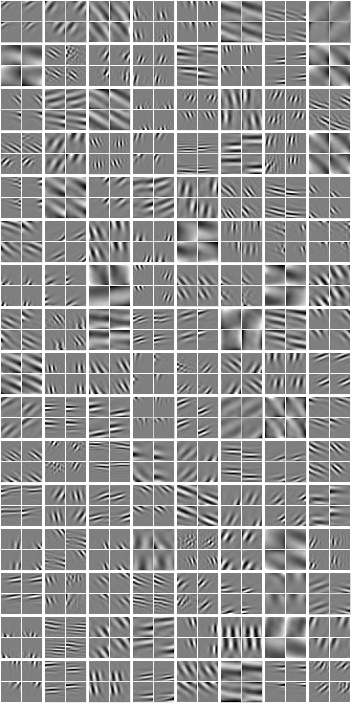
\includegraphics[scale=0.3]{./figures/SF_pool_SF.png} 
        %\end{center}
\end{columns} 
\end{frame} 

\begin{frame}
\frametitle{Slow Features Experiment \#4}    
\begin{columns}[c]
    \column{4cm}
        %\begin{center}
            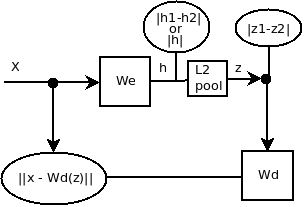
\includegraphics[scale=0.3]{./figures/sfa5.png} 
            \vspace{0.1cm}
             \begin{tiny}
			 Encoder: Linear \\
			 Decoder: Norm Linear \\
			 $L_2$-pooling: $z_{11} = \sqrt{\sum_{i=1} ^4 (W^e_i x)^2}$
			\end{tiny}
        %\end{center}
    \column{4cm}
        %\begin{center}
             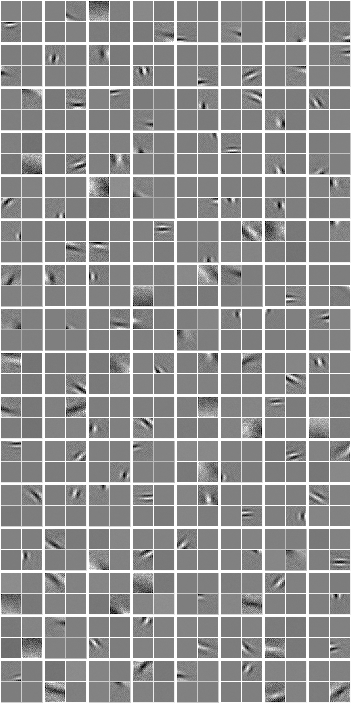
\includegraphics[scale=0.3]{./figures/dec_pooling.png} 
        %\end{center}
\end{columns} 
\end{frame} 


\begin{frame}
\frametitle{Input Data} 
  \begin{center}
             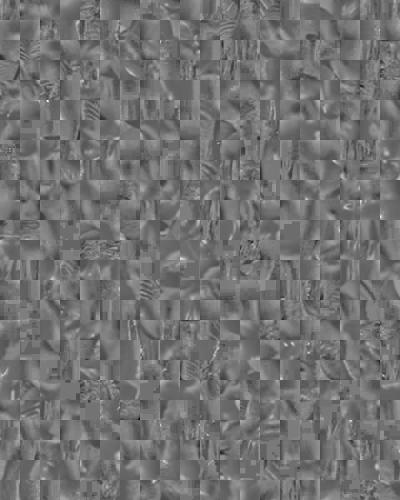
\includegraphics[scale=0.5]{./figures/input.png} 
    \end{center}
\end{frame} 

\begin{frame}
\frametitle{Linear Reconstruction} 
  \begin{center}
             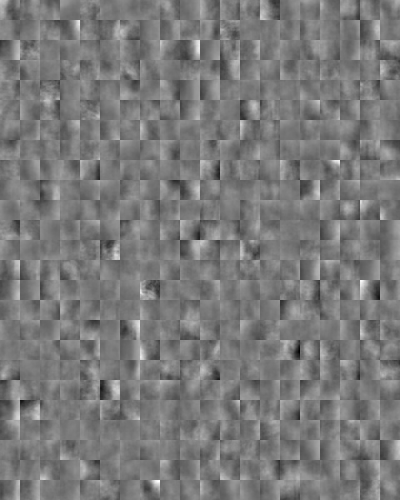
\includegraphics[scale=0.5]{./figures/pinv.png} 
    \end{center}
\end{frame} 

\begin{frame}
\frametitle{Input Data} 
  \begin{center}
             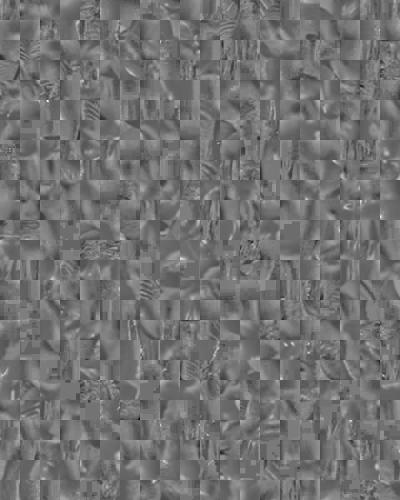
\includegraphics[scale=0.5]{./figures/input.png} 
    \end{center}
\end{frame} 

\begin{frame}
\frametitle{kNN-Code Space Reconstruction} 
  \begin{center}
             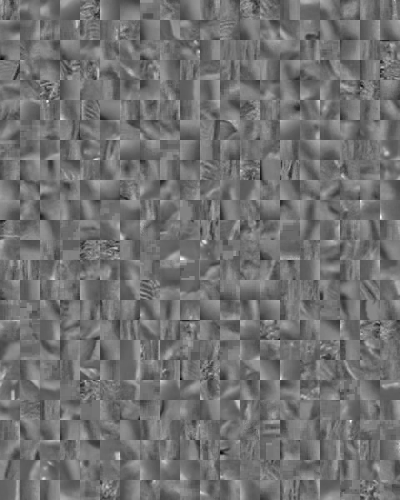
\includegraphics[scale=0.5]{./figures/znn.png} 
    \end{center}
\end{frame} 

\begin{frame}
\frametitle{kNN-Input Space Reconstruction} 
  \begin{center}
             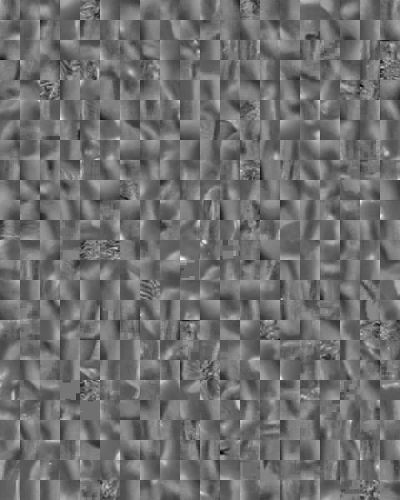
\includegraphics[scale=0.5]{./figures/xnn.png} 
    \end{center}
\end{frame} 

\begin{frame}
\frametitle{} 
  \begin{center}
             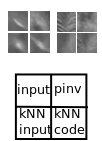
\includegraphics[scale=1]{./figures/example.png} 
    \end{center}
\end{frame} 

\begin{frame}
\frametitle{Curvature} 
\begin{itemize}
\item If we are after linearly equivariant features then it makes sense to minimize their curvature
\item This requires three samples: $\|2z_2 - z_1 - z_3\|$ 
\item We can also test the flatness of the representation and the quality of the decoder as follows: 
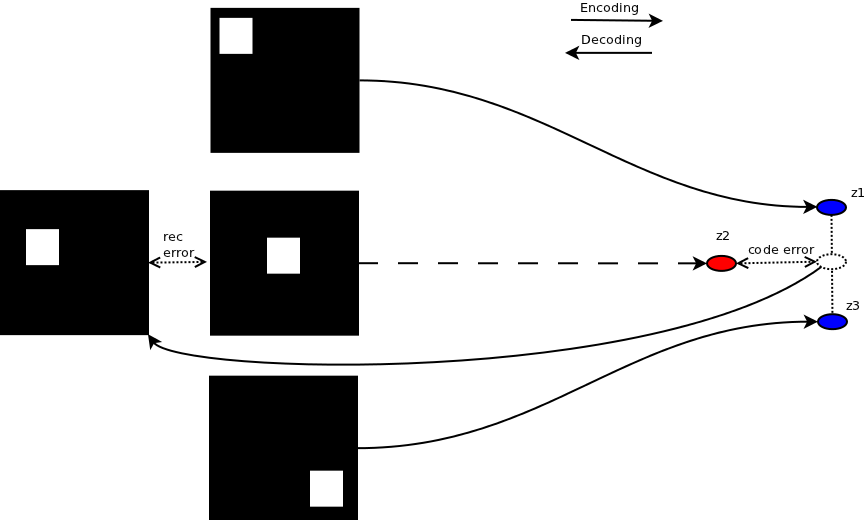
\includegraphics[scale=0.3]{./figures/testing.png} 
\end{itemize}
\end{frame} 

\begin{frame}
\centerline{
\huge
\emph{Thank You}} 
\vspace{10 mm} 
\centerline{
\huge
\emph{THE END}} 

\end{frame}

\end{document}


